%% Journal of Sports Sciences — Original Article — FIRST DRAFT (29 Oct 2026)
%% Author-date (APA-style) references via natbib + apalike. Same LaTeX setup as the A1/A3 drafts.

\documentclass[12pt,a4paper]{article}

\usepackage[utf8]{inputenc}
\usepackage[T1]{fontenc}
\usepackage{times}
\usepackage[margin=2.5cm]{geometry}
\usepackage{setspace}
\doublespacing

\usepackage{graphicx}
\graphicspath{{../figures/}}
\usepackage{float}
\usepackage{placeins}
\usepackage{amsmath,amssymb}
\usepackage{booktabs}
\usepackage{enumitem}
\usepackage[colorlinks=true,linkcolor=blue,citecolor=blue,urlcolor=blue]{hyperref}
\usepackage[round]{natbib}
\usepackage{lineno}
\linenumbers

\begin{document}

% ── Title page ──────────────────────────────────────────────

\begin{titlepage}
\vspace*{2cm}

{\noindent\LARGE\bfseries How much is the wind worth? Wind effects on sprint and horizontal-jump performance across age and ability in a national competition registry\par}

\vspace{1.5cm}

{\noindent\large
Atle G.\ Guttormsen$^{1,*}$ \\
\href{https://orcid.org/0000-0003-0188-8462}{ORCID: 0000-0003-0188-8462}
}

\vspace{0.8cm}

{\noindent
$^1$School of Economics and Business, Norwegian University of Life Sciences (NMBU), Ås, Norway
}

\vspace{0.8cm}

{\noindent
$^*$Corresponding author:\\
Atle G.\ Guttormsen\\
School of Economics and Business\\
Norwegian University of Life Sciences (NMBU)\\
P.O.\ Box 5003, 1432 Ås, Norway\\
E-mail: atle.guttormsen@nmbu.no
}

\vspace{1.2cm}

{\noindent\textbf{Running head:} Wind effects across age and ability}

\vspace{0.5cm}

{\noindent\textbf{Word count:} $\sim$2\,800 (main text, excluding abstract, references, tables, and figure legends)}

\end{titlepage}

% ── Abstract ────────────────────────────────────────────────

\newpage
\section*{Abstract}

\noindent Every empirical estimate of how wind affects track-and-field performance comes from elite seniors, yet wind rules --- the $\pm$2.0 m/s legality threshold above all --- apply identically to ten-year-olds and world-class sprinters. Using the Norwegian Athletics Federation's complete competition registry, which records gauge readings down to the youth 60 m, we estimated wind effects within athlete $\times$ season (79\,330 athlete-seasons; 433\,566 wind-measured results across five sprint and four horizontal-jump events, ages 10--34), with month and round controls and athlete-clustered errors. A +1 m/s tailwind was worth 0.059 s on 60 m, 0.082 s on 100 m, 0.121 s on 200 m, 2.9 cm in the long jump and 4.1 cm in the triple jump --- roughly double the published elite estimates, which our senior stratum reproduces as the endpoint of a gradient. The absolute effect declined monotonically with age (200 m, males: 0.144 s per m/s at 10--11 to 0.084 at 20--34) and with ability within age, scaling approximately with race duration; the percentage effect was much flatter but not constant. Headwinds cost more than tailwinds gave in sprints (100 m: 0.107 vs.\ 0.065 s per m/s, p $<$ 0.001). In class-specific short hurdles the estimates tracked flat sprints of the same distance. On the 100 m, a +2.0 m/s tailwind is worth 0.9--1.1 of a 12--13-year-old's own within-season standard deviation, against 0.5--0.8 among seniors, so uniform wind rules make youth results systematically noisier measures of ability than senior results.

\vspace{0.5em}
\noindent\textbf{Keywords:} wind; sprint; long jump; youth athletics; measurement; age-group competition; registry study

\newpage

% ════════════════════════════════════════════════════════════
\section{Introduction}

Wind is the one weather variable athletics regulates. Sprint and horizontal-jump results count for records only when tailwind does not exceed 2.0 m/s, gauge readings are part of the official result, and seasonal lists in many countries separate legal from wind-aided marks. How much the wind actually moves a result has been estimated in two ways: physical and quasi-physical models of the sprint \citep{linthorne1994,mureika2001}, and data-driven analyses of elite competition results \citep{moinat2018,hollings2012}. Both traditions agree on the order of magnitude for elite seniors --- roughly 0.04--0.06 s per m/s in the 100 m, somewhat more for women than for men --- and both concern elite seniors only. Reviews of sprint testing likewise treat wind as a condition to standardise, with correction factors derived from adult data \citep{haugen2016}.

Yet nothing guarantees that elite estimates transfer down the age and ability range, and the physics pulls in two directions. A slower runner spends longer on the course --- a 12-year-old needs roughly a third more time over 100 m than a senior --- so any given wind acts on them longer, inflating the absolute time effect. But aerodynamic drag scales with the square of airspeed, so slower runners spend a smaller share of their power against air, deflating it; children's higher surface-to-mass ratio pushes the other way again. The net scaling of the wind effect across age and ability is an empirical question that elite data cannot answer, and it matters practically: age-group records, seasonal youth lists, age-graded scoring tables and qualification standards all treat marks within $\pm$2.0 m/s as equivalent, in every age class, and talent evaluation leans on exactly these marks \citep{guttormsen2026development}.

The Norwegian registry is unusually well placed to answer it. Every sanctioned result in Norway is registered, and wind is measured and recorded down to the outdoor 60 m sprints that children contest from age 10 --- to our knowledge the only population-scale source of wind-measured sprint data on children. We pre-specified five questions: the direction of the effect within athlete and season (H1, a design check); how the absolute effect scales with age (H2 --- the exposure-time and aerodynamic-share mechanisms predict opposite directions); how the percentage effect scales (H3); whether headwinds cost more than tailwinds give (H4, as aerodynamics predicts); and what the $\pm$2.0 m/s window is worth in each class, expressed against athletes' own performance variability (H5). The analysis plan was committed to version control before estimation; the study was not externally preregistered. At the author's initiative after the main estimations, class-specific short hurdles were added as a documented extension.

% ════════════════════════════════════════════════════════════
\section{Methods}

\subsection{Data}

We used a frozen extract (29 October 2026) of the Norwegian Athletics Federation's results database, which is electronically complete from 2011. The main analysis covers all results from 2011 onwards in nine wind-measured events: 60 m, 80 m, 100 m, 150 m and 200 m sprints, and long jump, long jump from a take-off zone, triple jump and triple jump from a zone (the zone variants are youth events). The hurdles extension covers the ten short-hurdle event codes with substantive wind data (60 m to 110 m hurdles; each code specifies the class's hurdle height, so a code identifies an age-class specification). Only approved, outdoor, electronically timed results of athletes with known sex and birth year were analysed, at calendar-year ages 10--34, with event-specific plausibility bounds and wind readings within $\pm$8 m/s. Of 670\,803 extracted rows in the main events, 433\,566 entered the analysis (the largest exclusions being indoor results, principally indoor long jump, and 18\,692 outdoor rows without a wind value); the hurdles extension contributed 33\,386 rows. Times are analysed in seconds and jumps in metres (reported in centimetres); units were verified against known magnitudes per event.

\subsection{Statistical model}

The identifying variation is within athlete $\times$ season $\times$ event: the same athlete, in the same event and season, racing under different winds. For each event we estimated
\[
y_{it} = \alpha_{i(\text{athlete} \times \text{year})} + \beta \cdot \text{wind}_{it} + \text{month dummies} + \text{round dummies} + \varepsilon_{it},
\]
by within-demeaning, with standard errors clustered on athlete; 79\,330 athlete-seasons contribute at least two wind-measured results. $\beta$ is reported as the \emph{gain per +1 m/s of tailwind}, in seconds or centimetres, and in percent from a log-outcome specification. Age-band (10--11 through 20--34) and sex-specific models address H2/H3; within-group ability tertiles (athlete-season mean performance, standardised within event $\times$ sex $\times$ age band) address ability scaling; separate slopes for head- and tailwind address H4; a quadratic term probes curvature. For H5, the advantage of a +2.0 m/s tailwind over still air is expressed in seconds and as a share of the within-athlete-season standard deviation of performance in the same event, sex and age band. Pre-specified robustness analyses required at least three results per cell, excluded readings of exactly 0.0, split the period (2011--2019 vs.\ 2021--2026), replaced month dummies with meet fixed effects (two-way demeaning), and clustered on meet. Analyses used Python 3.13 (pandas, statsmodels).

Two interpretive rules were fixed in advance. First, a single gauge reading over 10--13 s does not measure the wind each athlete met; this measurement error attenuates estimates toward zero, so all effects are read as lower bounds. Second, wind is not randomly assigned: identification relies on within-season comparisons with month, round and (in robustness) meet controls, and no causal language beyond this design sense is used. For the jumps, one further caveat applies: the registry stores the wind of the measured (best) attempt, so jump estimates may contain an attempt-selection component that sprint estimates, with one time per race, do not.

\subsection{Ethics and transparency}

The data are public competition results; no athlete is identified. Performance data below age 13 are used solely to estimate measurement conditions --- not to rank, list or evaluate children --- in keeping with the purpose of the Norwegian children's sport regulations. The project falls outside the Norwegian Health Research Act; an assessment from Sikt was obtained. The analysis plan was committed to version control before estimation; code and aggregate outputs are available, and athlete-level files are regenerable from the registry. Reporting follows STROBE where applicable \citep{vonelm2007}.

% ════════════════════════════════════════════════════════════
\section{Results}

\subsection{Sample and wind exposure}

Table~\ref{tab:sample} describes the nine main events. Wind readings centred near calm with wide spread (median +0.3 m/s; 5th--95th percentile $-$2.0 to +2.7); 9.5\,\% of readings were exactly 0.0 and 17\,\% fell on whole metres per second, indicating only mild digit preference. The bulk of the material is young: the 60 m, contested outdoors by the youngest classes, is the largest single event (103\,377 analysed results, of which 72\,669 lie in athlete-seasons with at least two wind-measured races and thus contribute to estimation).

\begin{table}[H]
\centering
\caption{Analysed events: volume, marks, and wind exposure (2011--2026).}
\label{tab:sample}
\footnotesize
\begin{tabular}{lcccccc}
\toprule
Event & Results & In cells $\geq$2 & Athlete-seasons & Athletes & Median mark & Wind, median (p5--p95) \\
\midrule
60 m & 103\,377 & 72\,669 & 19\,374 & 10\,799 & 9.59 s & +0.1 ($-$2.3--+2.5) \\
80 m & 5\,795 & 1\,410 & 620 & 466 & 12.53 s & +0.0 ($-$2.6--+2.5) \\
100 m & 76\,598 & 64\,756 & 13\,253 & 5\,468 & 12.88 s & +0.4 ($-$2.2--+2.8) \\
150 m & 2\,154 & 334 & 153 & 127 & 19.64 s & +0.3 ($-$2.5--+2.2) \\
200 m & 76\,261 & 59\,416 & 15\,571 & 6\,621 & 27.99 s & +0.4 ($-$2.2--+2.9) \\
Long jump & 85\,789 & 51\,870 & 12\,204 & 6\,404 & 4.05 m & +0.4 ($-$1.6--+2.6) \\
Long jump (zone) & 54\,665 & 44\,336 & 12\,338 & 7\,835 & 3.64 m & +0.3 ($-$1.7--+2.7) \\
Triple jump & 21\,067 & 15\,071 & 3\,956 & 2\,087 & 9.67 m & +0.6 ($-$1.3--+2.8) \\
Triple jump (zone) & 7\,860 & 5\,426 & 1\,861 & 1\,413 & 8.42 m & +0.4 ($-$1.5--+2.8) \\
\bottomrule
\end{tabular}
\vspace{0.3em}
\parbox{0.95\textwidth}{\footnotesize Counts are analysed rows (approved, outdoor, electronic, ages 10--34, wind within $\pm$8 m/s). Exact values per event are in the deposited tables; this table's counts and wind summaries are computed from the analysis file.}
\end{table}

\subsection{What a metre per second is worth (H1)}

Table~\ref{tab:main} reports the main within-athlete estimates. A +1 m/s tailwind was worth 0.059 s (95\,\% CI 0.058--0.060) on 60 m, 0.082 s (0.081--0.084) on 100 m, 0.121 s (0.118--0.125) on 200 m, 2.9 cm (2.7--3.1) in the long jump and 4.1 cm (3.6--4.6) in the triple jump; in percentage terms, 0.40--0.65\,\% per m/s. All directions matched H1. The small 80 m and 150 m events gave consistent estimates with wide intervals.

\begin{table}[H]
\centering
\caption{Gain per +1 m/s of tailwind, within athlete $\times$ season.}
\label{tab:main}
\small
\begin{tabular}{lcccc}
\toprule
Event & Gain per +1 m/s (95\,\% CI) & Percent per +1 m/s (95\,\% CI) & n & Athlete-seasons \\
\midrule
60 m & 0.059 s (0.058--0.060) & 0.625 (0.613--0.637) & 72\,669 & 19\,374 \\
80 m & 0.075 s (0.064--0.085) & 0.630 (0.547--0.713) & 1\,410 & 620 \\
100 m & 0.082 s (0.081--0.084) & 0.646 (0.635--0.656) & 64\,756 & 13\,253 \\
150 m & 0.081 s (0.049--0.114) & 0.467 (0.292--0.642) & 334 & 153 \\
200 m & 0.121 s (0.118--0.125) & 0.442 (0.429--0.454) & 59\,416 & 15\,571 \\
Long jump & 2.88 cm (2.70--3.07) & 0.641 (0.595--0.686) & 51\,870 & 12\,204 \\
Long jump (zone) & 2.11 cm (1.96--2.27) & 0.570 (0.527--0.614) & 44\,336 & 12\,338 \\
Triple jump & 4.10 cm (3.64--4.55) & 0.398 (0.352--0.445) & 15\,071 & 3\,956 \\
Triple jump (zone) & 3.88 cm (3.05--4.71) & 0.449 (0.351--0.548) & 5\,426 & 1\,861 \\
\bottomrule
\end{tabular}
\end{table}

These population-level effects are roughly double the published elite estimates. That is not a contradiction but a continuum: restricted to seniors (20--34), our 100 m estimate falls to 0.071 s per m/s for men and 0.072 for women --- and our senior men, averaging about 11.4 s on the 100 m, are themselves slower than the elite samples behind the published figures of roughly 0.04--0.05 s per m/s \citep{linthorne1994,moinat2018}. The elite literature, it turns out, has been describing the fast end of a gradient.

\subsection{The effect falls with age --- and with speed (H2, H3)}

Figure~\ref{fig:age} and Table~\ref{tab:age} show the core result. In absolute seconds, the wind effect declined monotonically with age in every sprint and both sexes: on 200 m for boys and men from 0.144 s per m/s at 10--11 to 0.084 at 20--34; on 60 m from 0.070 at 10--11 to 0.041 at 16--17; on 100 m from 0.101 at 12--13 to 0.071 at 20--34. The exposure-time mechanism wins: mean race durations shrink in almost the same proportion (men's 100 m, 14.96 s at 12--13 vs.\ 11.42 s at 20--34, a ratio of 1.31, against a wind-effect ratio of 1.42), so the percentage effect (Figure~\ref{fig:agepct}) is far flatter --- but not constant, declining for instance from 0.70 to 0.62\,\% per m/s on the men's 100 m and from 0.70 to 0.52\,\% on the 60 m. Within age bands, the same logic reappears across ability (Figure~\ref{fig:level}): the lowest ability tertile gained most per m/s in every sprint (100 m: 0.087 vs.\ 0.078 s in the highest tertile). Slower athletes --- whether young or simply weaker --- are exposed longer, and no single correction factor, absolute or proportional, is exactly age-invariant.

\begin{figure}[H]
\centering
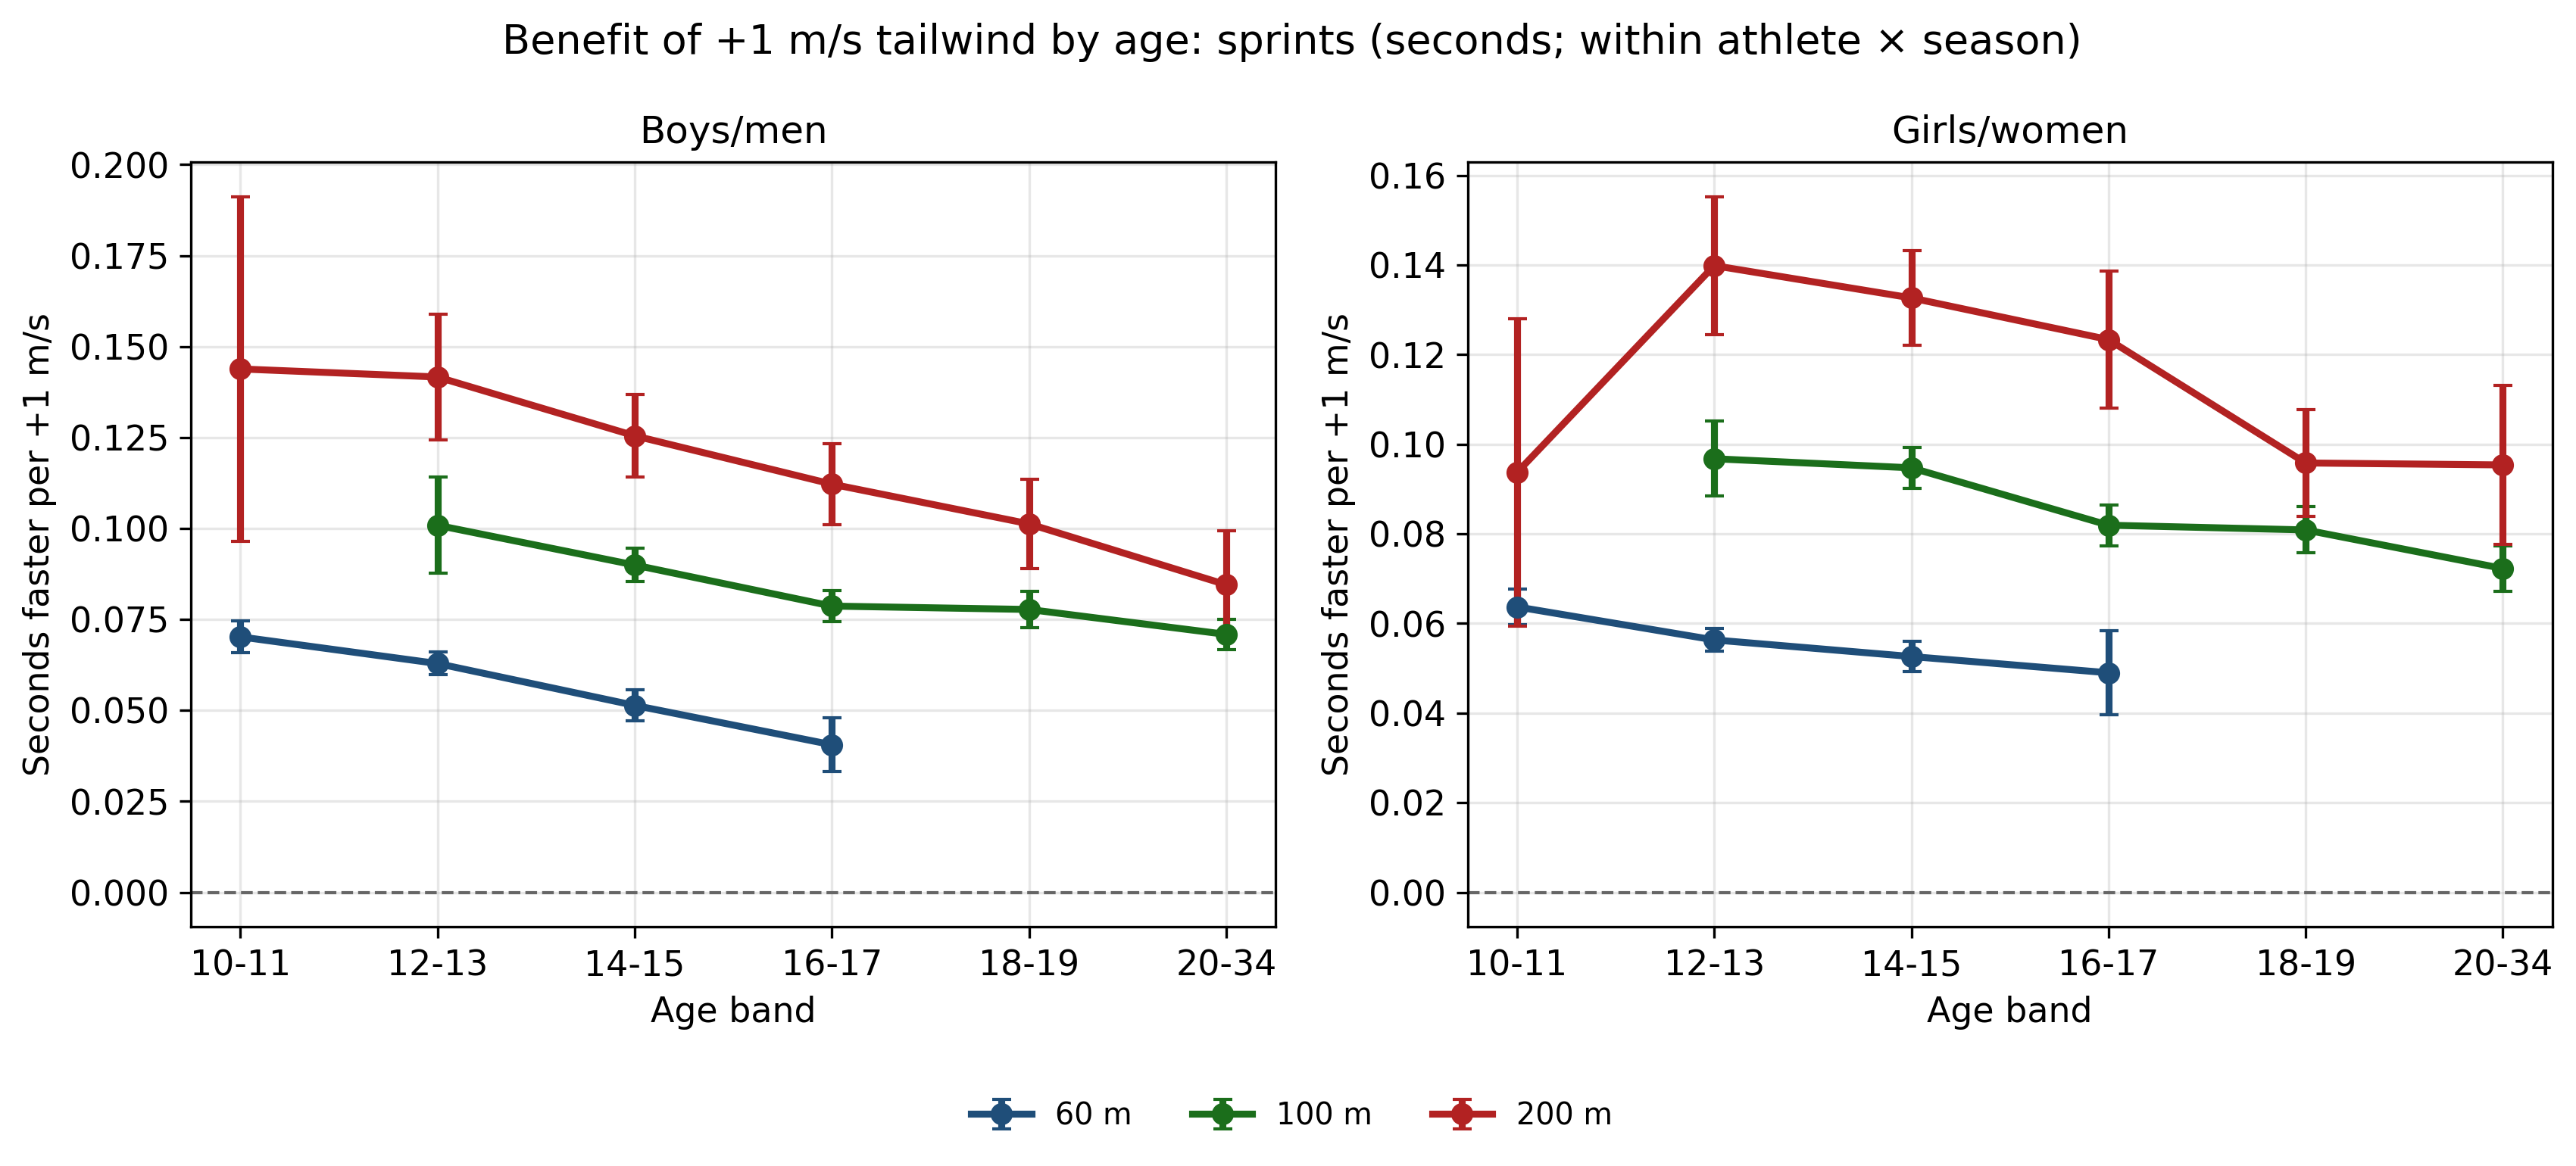
\includegraphics[width=\textwidth]{fig1_effect_by_age.png}
\caption{Benefit of +1 m/s tailwind by age band, in seconds, for sprints (within athlete $\times$ season; 95\,\% CIs).}
\label{fig:age}
\end{figure}

\begin{figure}[H]
\centering
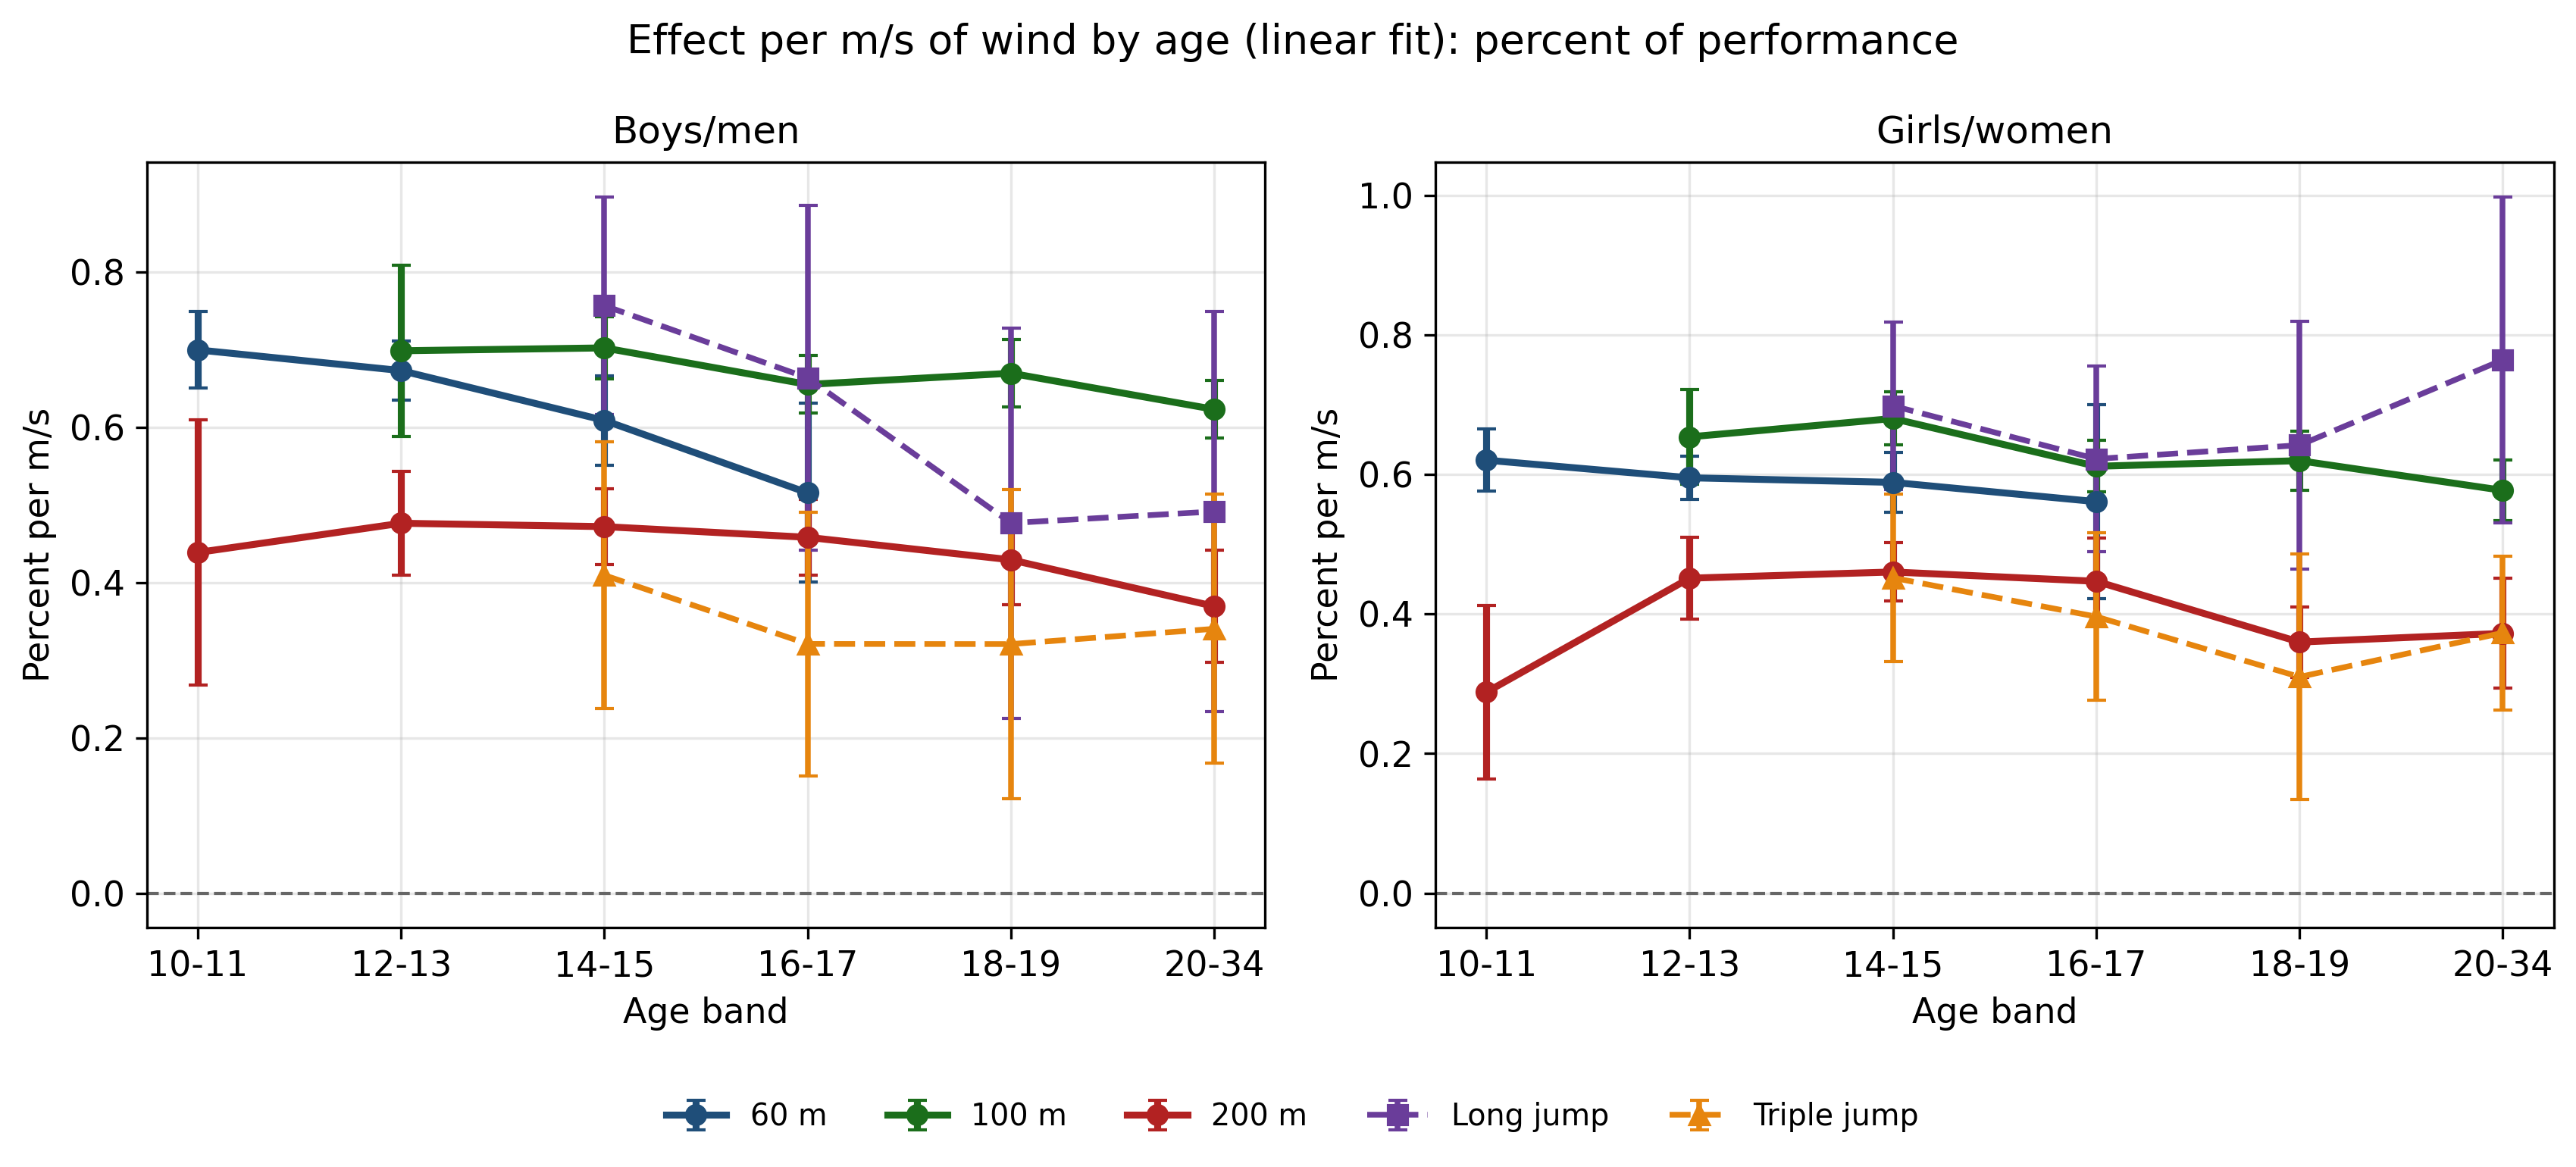
\includegraphics[width=\textwidth]{fig2_effect_by_age_pct.png}
\caption{The same scaling in percent of performance. The percentage effect is far flatter across age than the absolute effect, but still declines.}
\label{fig:agepct}
\end{figure}

\begin{table}[H]
\centering
\caption{Gain per +1 m/s of tailwind (seconds, 95\,\% CI) by age band and sex, sprints.}
\label{tab:age}
\footnotesize
\begin{tabular}{llcccccc}
\toprule
Event & Sex & 10--11 & 12--13 & 14--15 & 16--17 & 18--19 & 20--34 \\
\midrule
60 m & Boys/men & 0.070 (0.066--0.075) & 0.063 (0.060--0.065) & 0.051 (0.048--0.054) & 0.041 (0.032--0.049) & --- & --- \\
60 m & Girls/women & 0.064 (0.060--0.068) & 0.056 (0.054--0.058) & 0.053 (0.050--0.055) & 0.049 (0.041--0.057) & --- & --- \\
100 m & Boys/men & --- & 0.101 (0.086--0.116) & 0.090 (0.086--0.094) & 0.079 (0.075--0.082) & 0.078 (0.073--0.083) & 0.071 (0.067--0.074) \\
100 m & Girls/women & --- & 0.097 (0.087--0.106) & 0.095 (0.091--0.098) & 0.082 (0.078--0.086) & 0.081 (0.076--0.085) & 0.072 (0.069--0.076) \\
200 m & Boys/men & 0.143 (0.095--0.192) & 0.141 (0.125--0.158) & 0.125 (0.115--0.135) & 0.112 (0.103--0.121) & 0.101 (0.091--0.111) & 0.084 (0.076--0.093) \\
200 m & Girls/women & 0.094 (0.056--0.131) & 0.140 (0.128--0.151) & 0.133 (0.124--0.142) & 0.124 (0.113--0.134) & 0.096 (0.086--0.106) & 0.095 (0.084--0.107) \\
\bottomrule
\end{tabular}
\vspace{0.2em}
\parbox{0.97\textwidth}{\footnotesize Dashes: the event is not contested outdoors in that class (60 m above 17) or data are sparse (100 m at 10--11, where 60 m is the standard sprint). Table values are reproduced from the deposited estimation files.}
\end{table}

\begin{figure}[H]
\centering
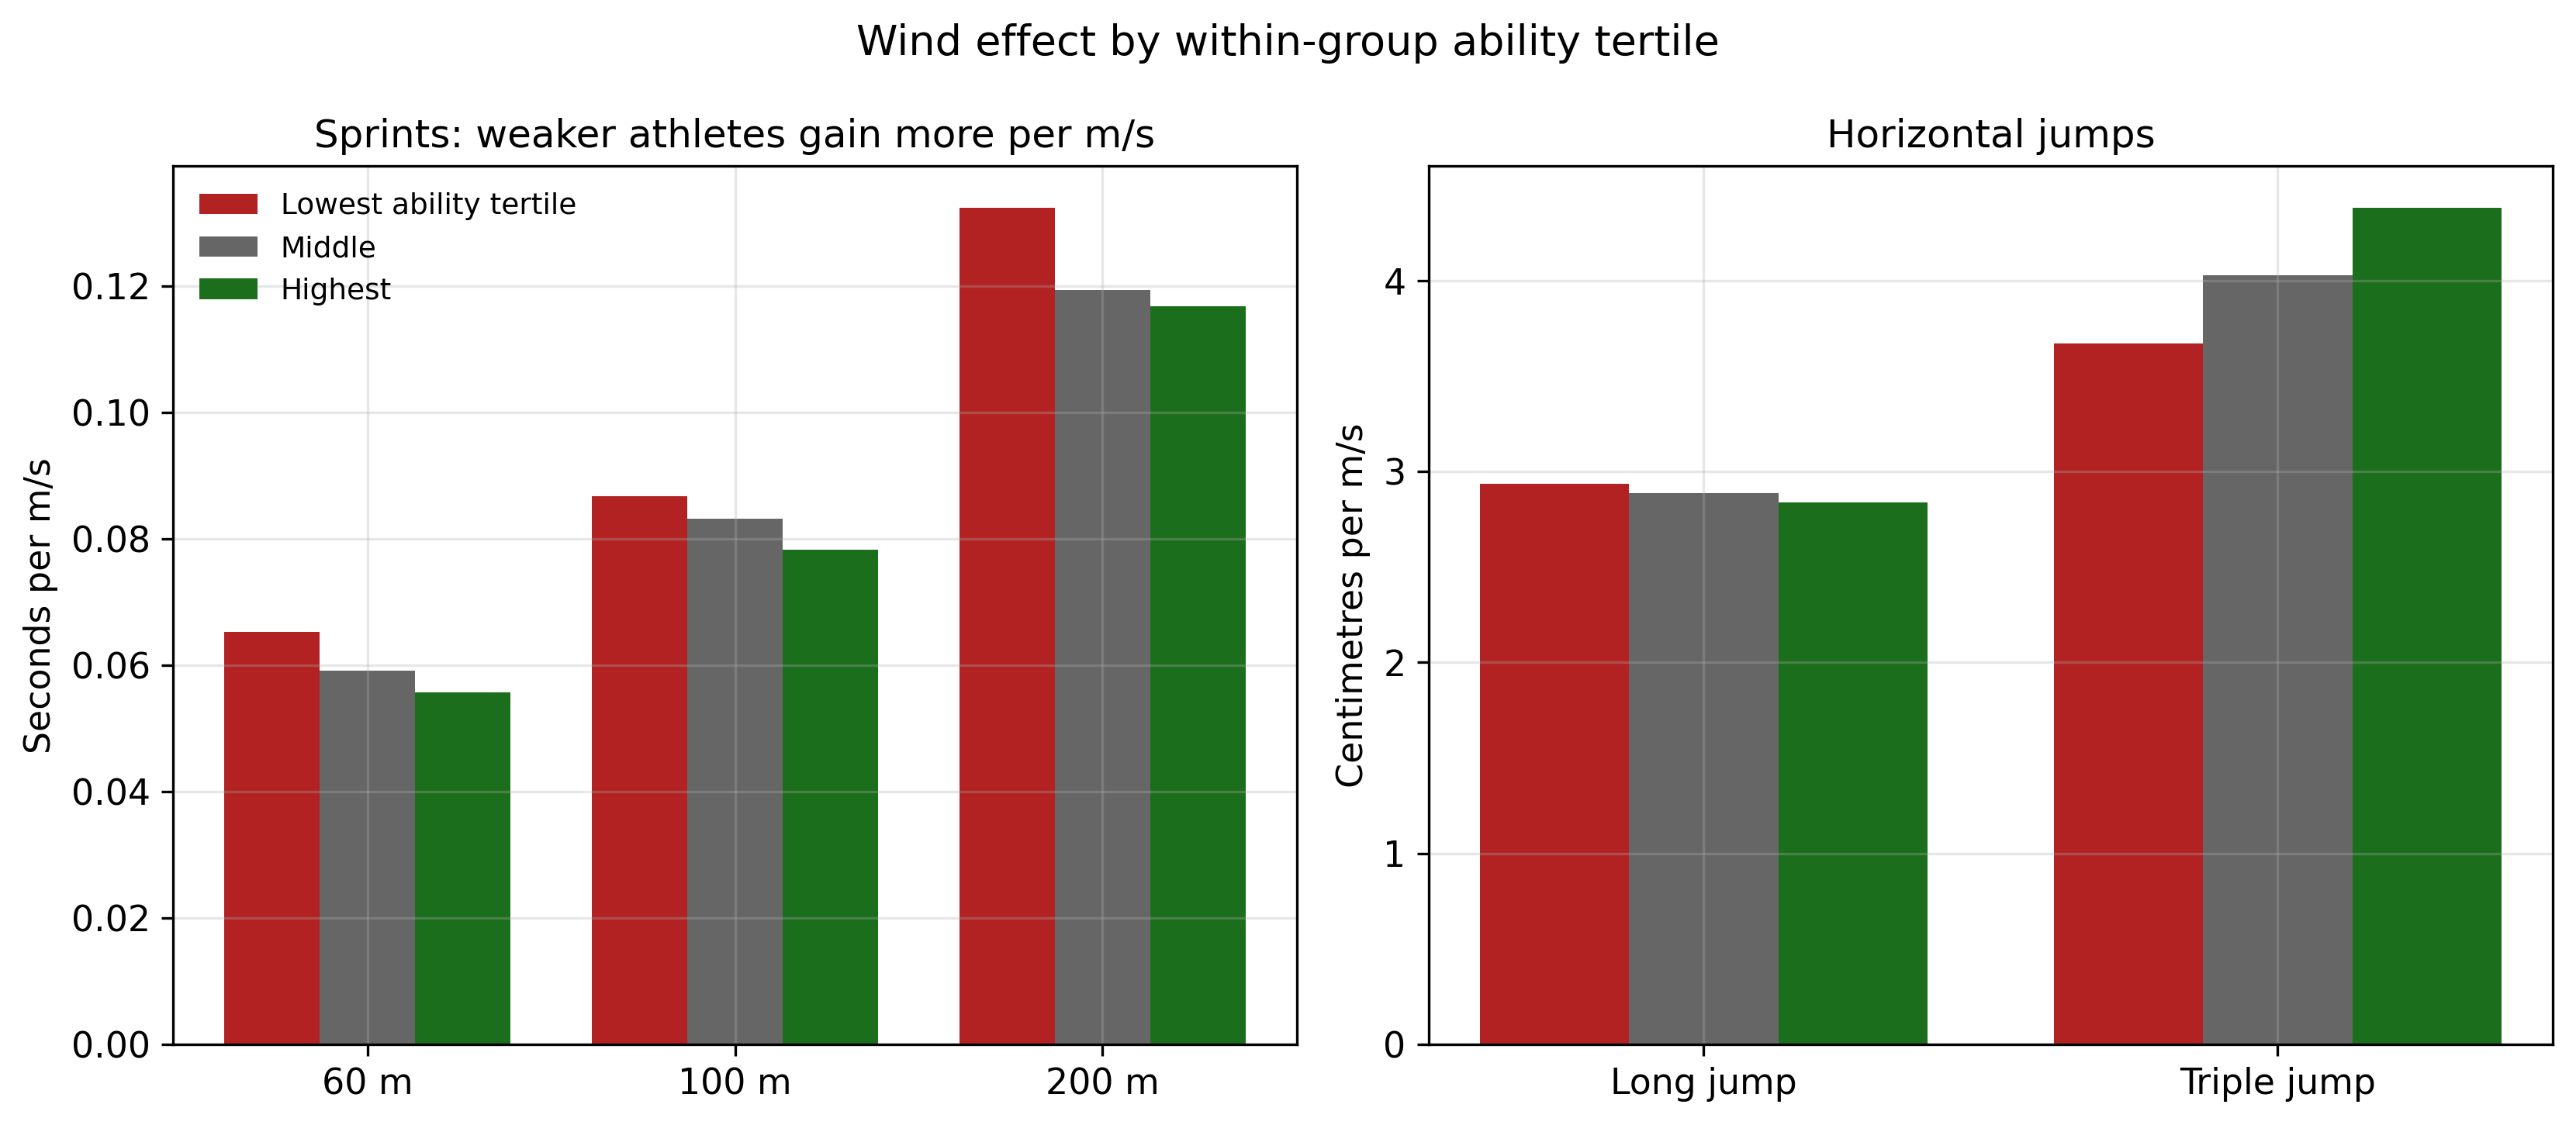
\includegraphics[width=\textwidth]{fig4_level.png}
\caption{Wind effect by within-group ability tertile (ability defined within event $\times$ sex $\times$ age band).}
\label{fig:level}
\end{figure}

\subsection{Headwinds cost more than tailwinds give (H4)}

In every large sprint event the headwind slope exceeded the tailwind slope (Figure~\ref{fig:asym}): on 100 m a $-$1 m/s headwind cost 0.107 s against a +1 m/s tailwind's 0.065 s (p $<$ 0.001 for equal slopes); on 200 m, 0.184 against 0.078; on 60 m, 0.072 against 0.048. The positive quadratic terms tell the same story (200 m: +0.0141 s per (m/s)$^2$, SE 0.0007). Both match the physics of drag rising with the square of airspeed. In the jumps the asymmetry was absent (long jump, p = 0.999) or reversed in the zone and triple-jump variants --- a pattern consistent with attempt selection, since the recorded wind belongs to the best attempt, and best attempts are more often wind-assisted.

\begin{figure}[H]
\centering
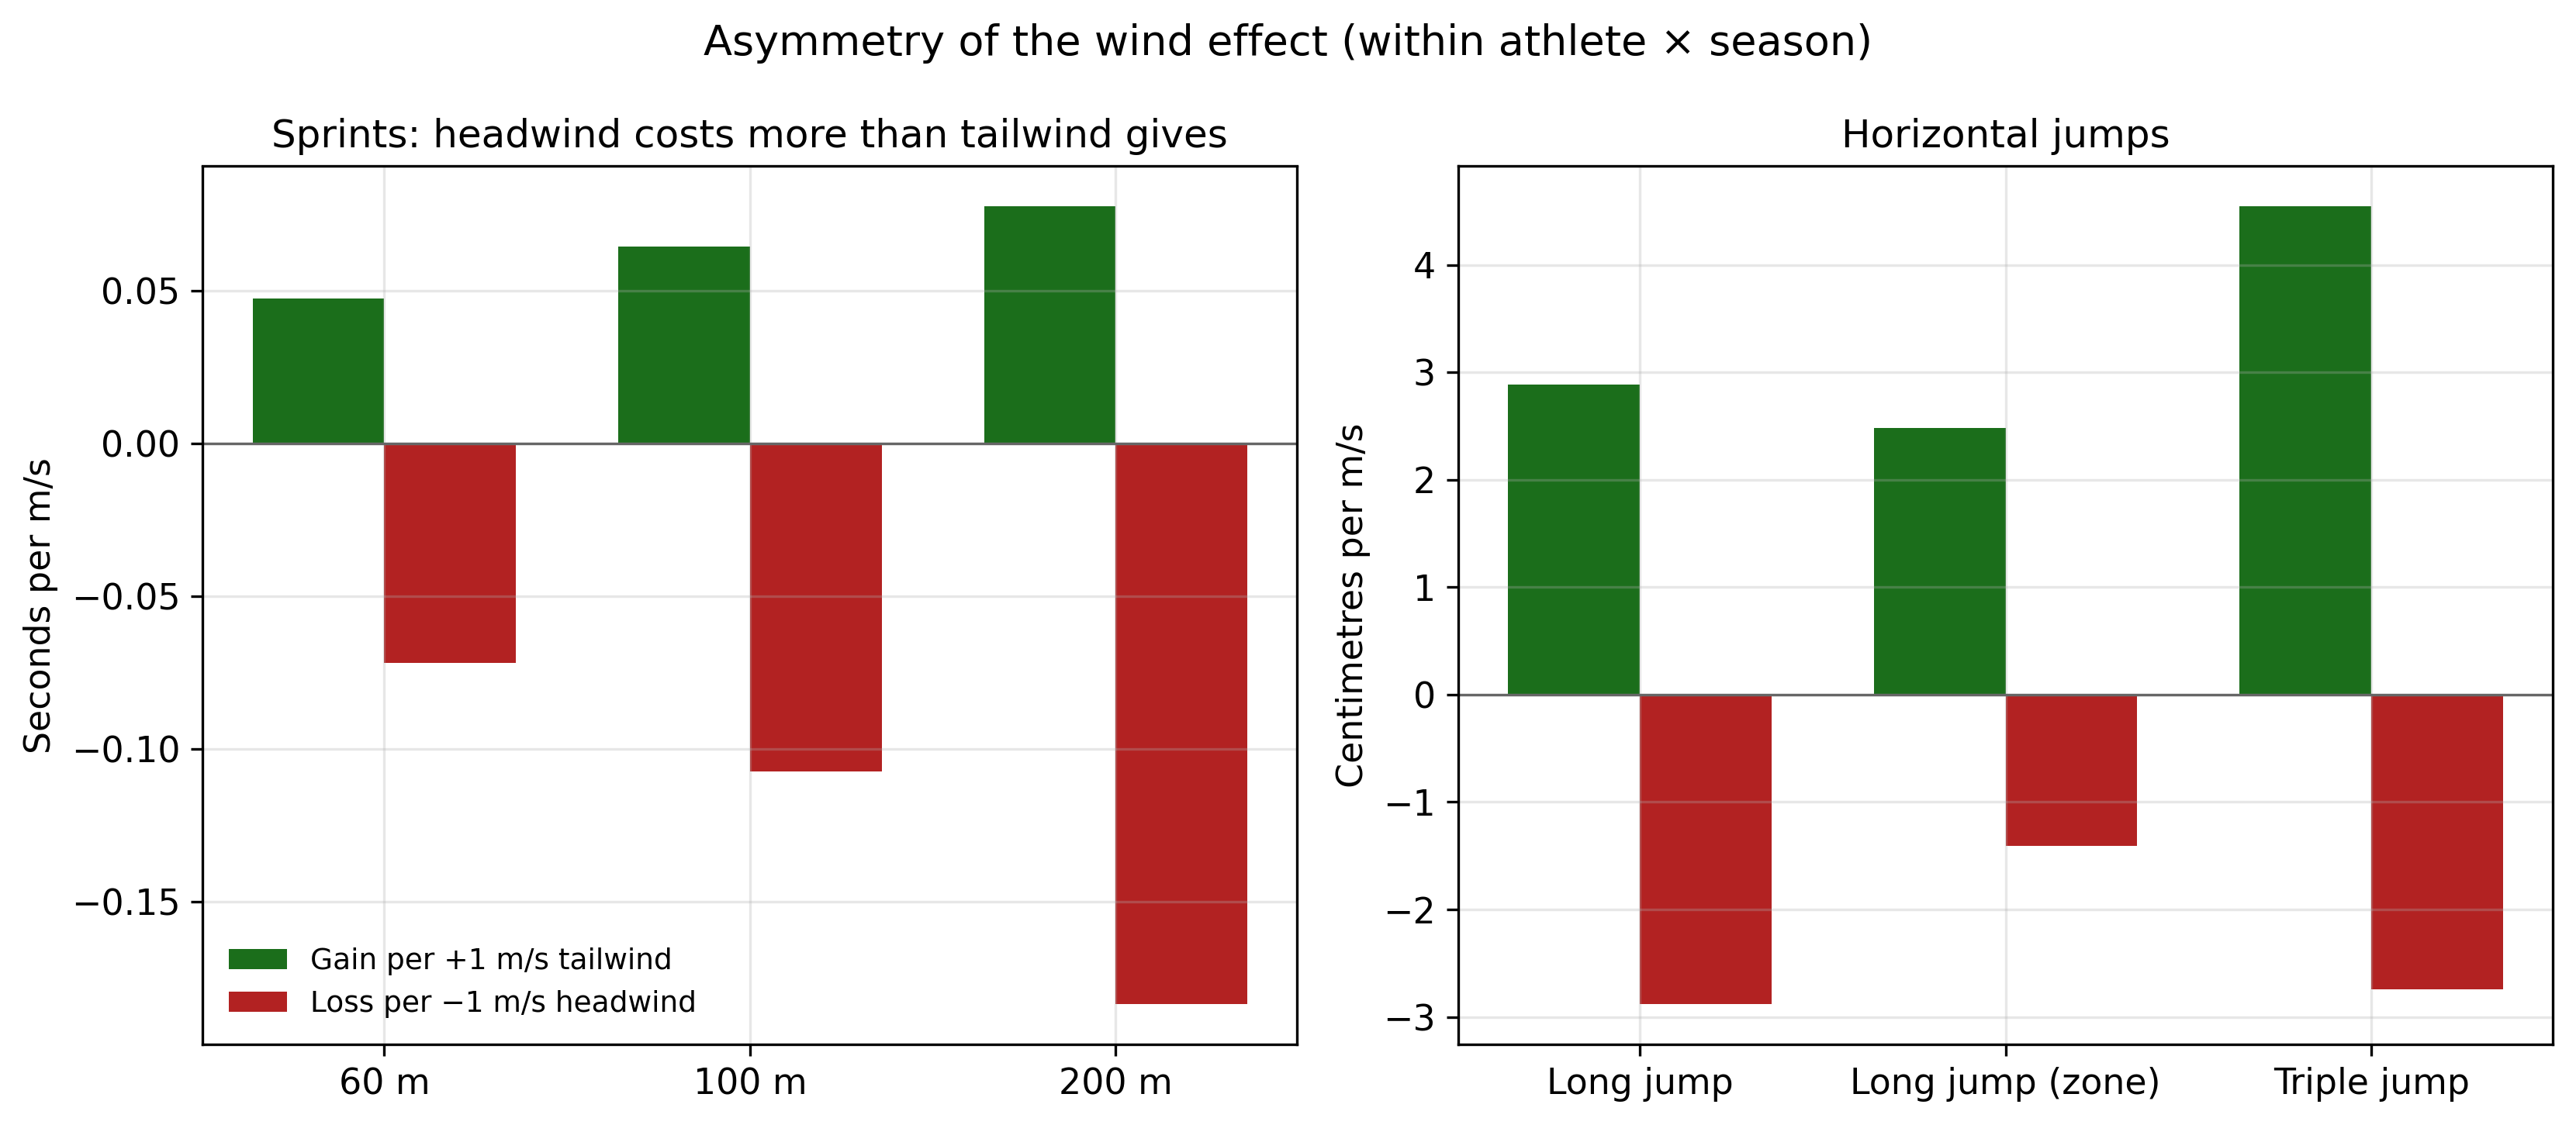
\includegraphics[width=\textwidth]{fig3_asymmetry.png}
\caption{Separate head- and tailwind slopes (within athlete $\times$ season).}
\label{fig:asym}
\end{figure}

\subsection{Short hurdles behave like flat sprints of their distance}

In the user-facing age-class system, hurdle events carry class-specific heights, so each event code identifies an age-class specification. Across the ten codes with wind data (Table~\ref{tab:hurdles}; Figure~\ref{fig:hurdles}), estimates tracked flat sprints of the same distance and class: the youth 60 m hurdles at 0.062--0.063 s per m/s against 0.056--0.070 for the flat 60 m in the same bands, with point estimates in the 100/110 m hurdles 10--30\,\% above the flat references but with overlapping intervals. The age gradient reappeared within a distance: on the 100 m hurdles, 0.108 s per m/s for the 76.2 cm specification contested at 16--17 against 0.069 for the senior women's 84 cm event.

\begin{table}[H]
\centering
\caption{Wind effect in short hurdles by class-specific event code (sex-specific rows; flat-sprint reference at the same distance class and modal age band).}
\label{tab:hurdles}
\footnotesize
\begin{tabular}{llcccc}
\toprule
Event (hurdle height) & Sex & Modal band & Gain per +1 m/s (95\,\% CI), s & Flat ref., s & n \\
\midrule
60 m hurdles 68 cm & Boys & 10--11 & 0.055 (0.035--0.076) & 0.070 & 1\,215 \\
60 m hurdles 68 cm & Girls & 10--11 & 0.067 (0.052--0.082) & 0.064 & 2\,562 \\
60 m hurdles 76.2 cm & Boys & 12--13 & 0.063 (0.049--0.076) & 0.063 & 3\,457 \\
60 m hurdles 76.2 cm & Girls & 12--13 & 0.062 (0.052--0.072) & 0.056 & 7\,293 \\
80 m hurdles 76.2 cm & Girls & 14--15 & 0.072 (0.055--0.089) & --- & 2\,529 \\
80 m hurdles 84 cm & Boys & 14--15 & 0.078 (0.056--0.099) & --- & 1\,474 \\
100 m hurdles 76.2 cm & Girls & 16--17 & 0.108 (0.090--0.127) & 0.082 & 1\,055 \\
100 m hurdles 84 cm & Women & 20--34 & 0.069 (0.041--0.097) & 0.072 & 2\,882 \\
100 m hurdles 91.4 cm & Boys & 16--17 & 0.084 (0.054--0.113) & 0.079 & 685 \\
110 m hurdles 91.4 cm & Boys & 16--17 & 0.103 (0.035--0.171) & 0.079 & 583 \\
110 m hurdles 100 cm & Men & 18--19 & 0.096 (0.060--0.133) & 0.078 & 657 \\
110 m hurdles 106.7 cm & Men & 20--34 & 0.085 (0.042--0.128) & 0.071 & 623 \\
\bottomrule
\end{tabular}
\vspace{0.2em}
\parbox{0.95\textwidth}{\footnotesize The hurdles analysis was added after the main estimations at the author's initiative and is documented as a post-plan extension. Flat references are the 60 m or 100 m estimate for the same sex and modal age band.}
\end{table}

\begin{figure}[H]
\centering
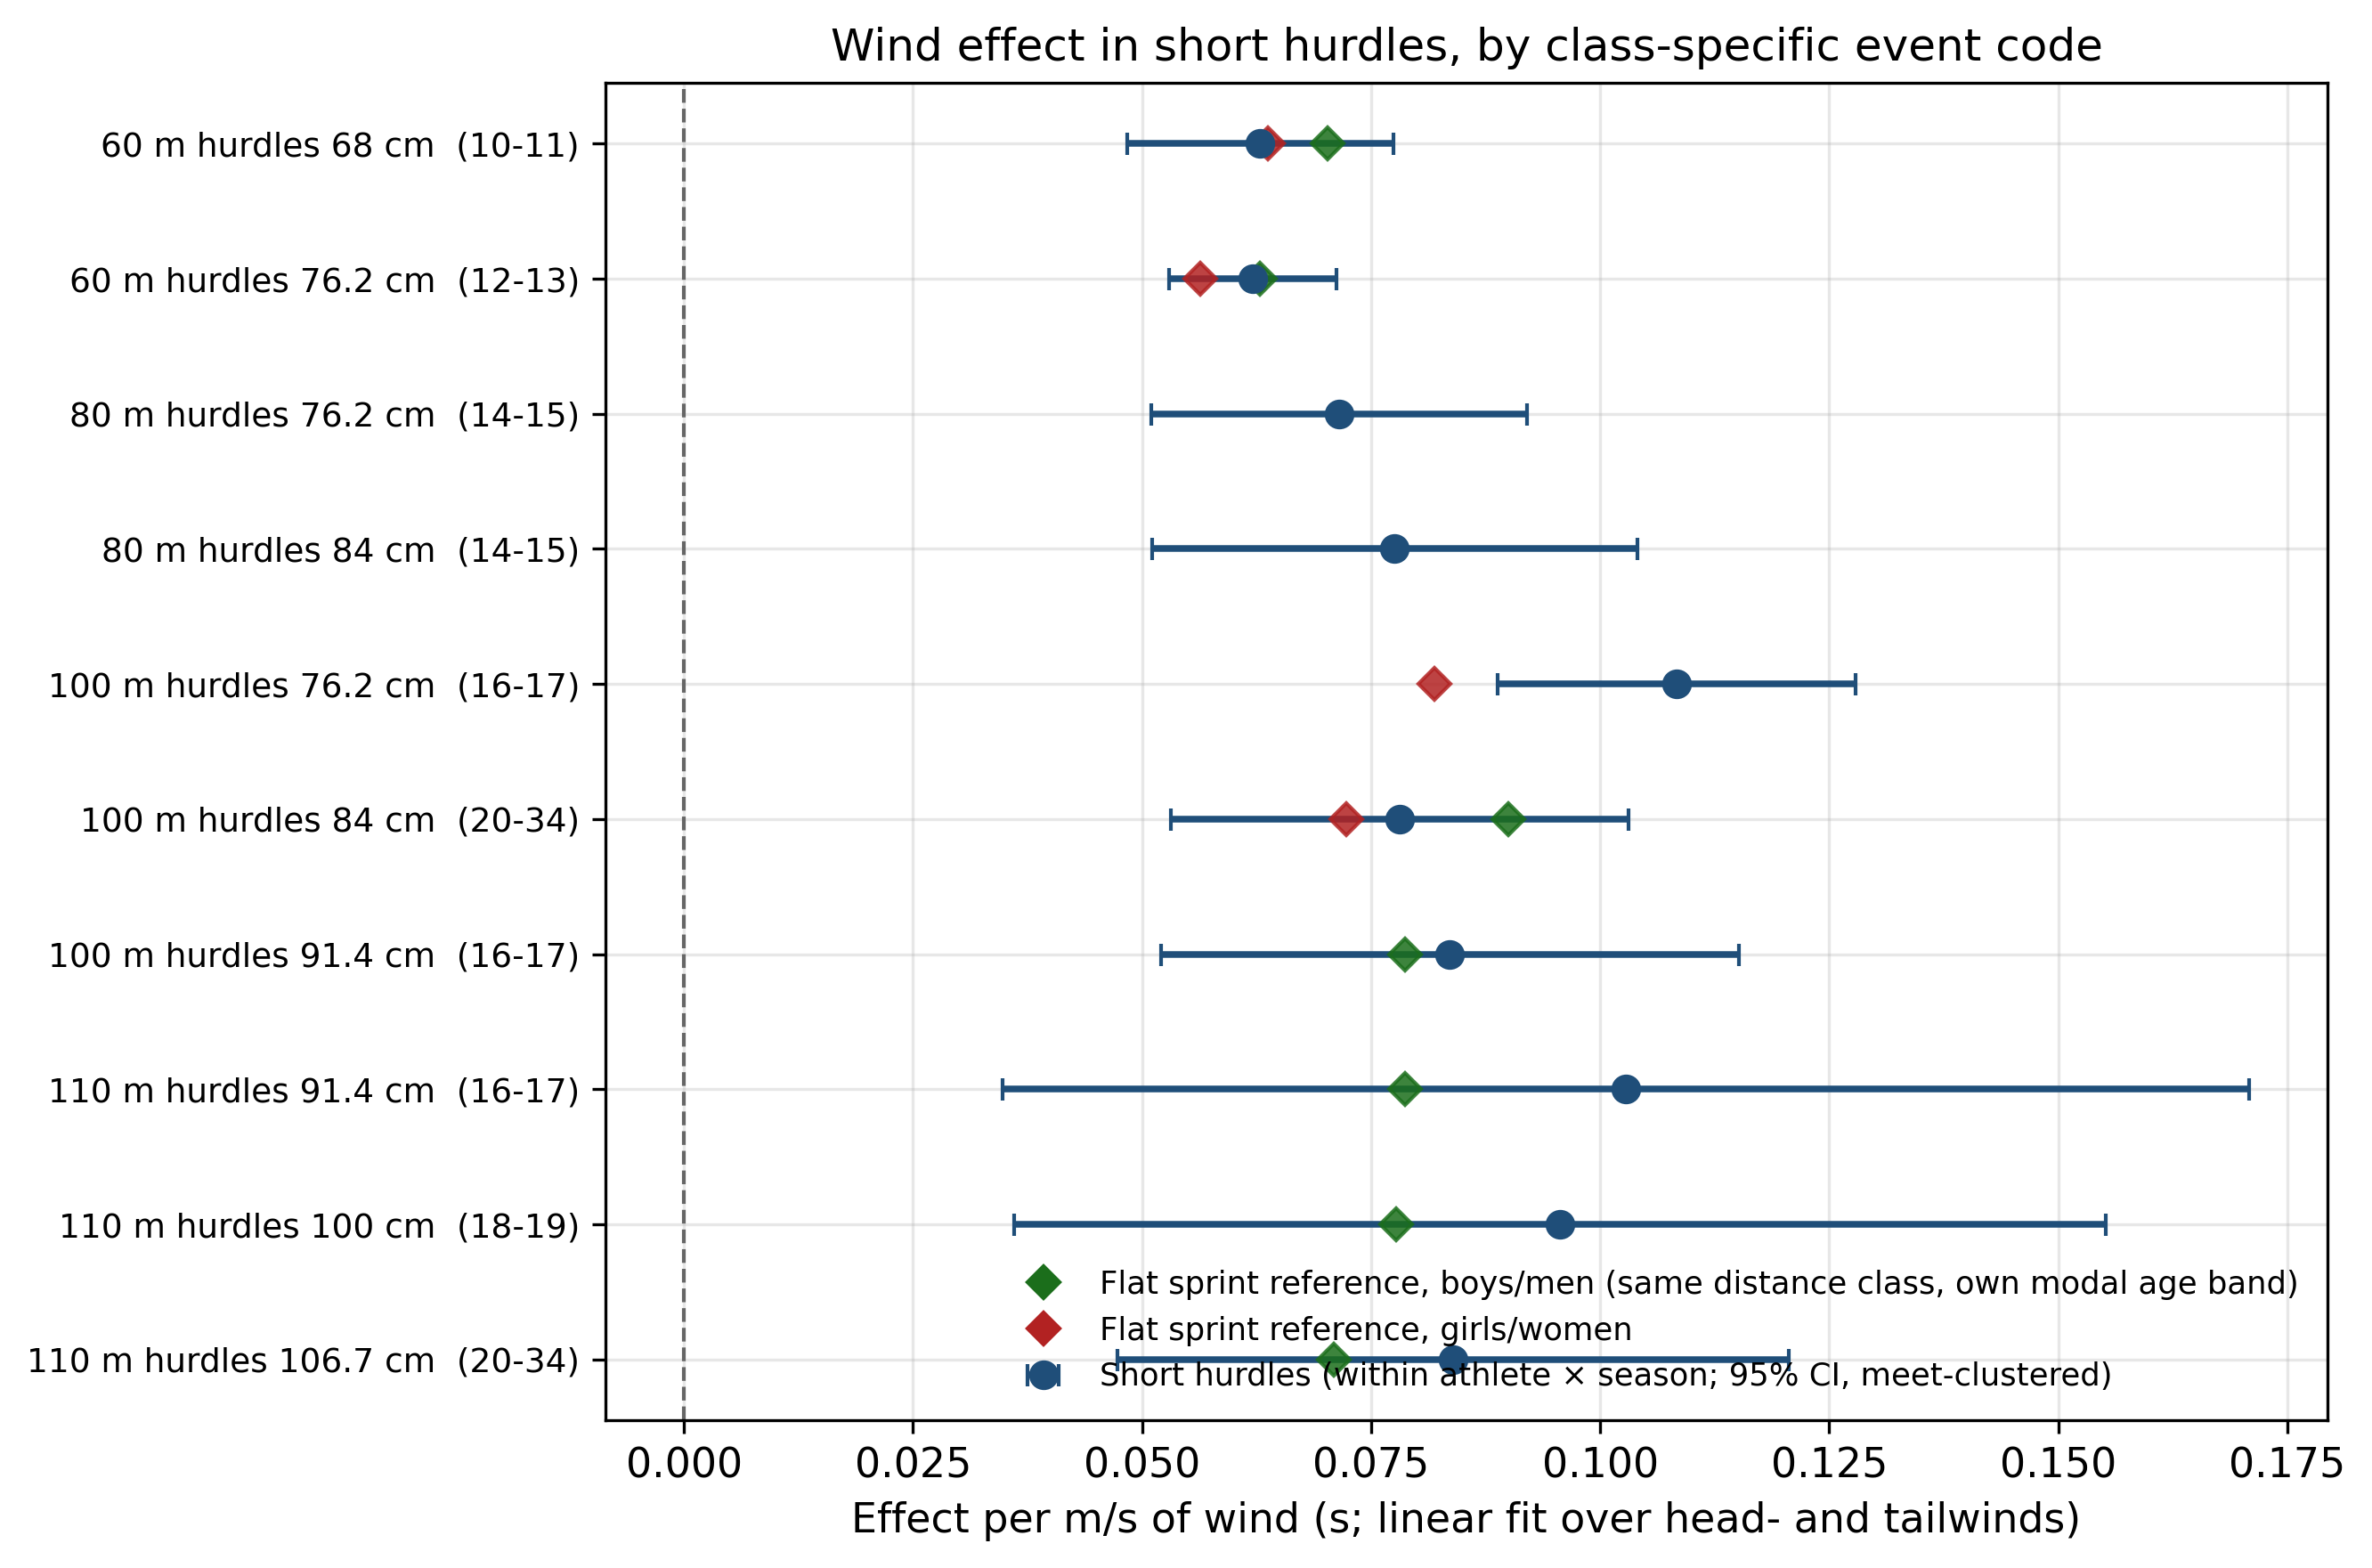
\includegraphics[width=0.95\textwidth]{fig5_hurdles.png}
\caption{Short hurdles: wind effect per class-specific code (pooled sexes; dots with 95\,\% CIs) against flat-sprint references (diamonds).}
\label{fig:hurdles}
\end{figure}

\subsection{What the legal window is worth in each class (H5)}

Table~\ref{tab:window} translates the estimates into the quantity the rules regulate: the advantage of a +2.0 m/s tailwind over still air, expressed in seconds and as a share of the athlete's own within-season performance variability. For boys at 12--13, +2.0 m/s is worth 0.20 s on the 100 m --- 0.88 within-athlete standard deviations; for girls, 0.19 s and 1.07 SD. Among seniors the same window is worth 0.14 s and roughly half a standard deviation for men (0.58) and four-fifths for women (0.81). On the 100 m the legal range thus spans about one unit of a young athlete's own typical variation against one half to four fifths among seniors: under identical rules, youth marks are intrinsically noisier measures of ability. On the 60 m and 200 m the seconds decline with age in the same way, while the SD shares move less systematically (Table~\ref{tab:window}), because within-season performance variability itself shrinks with age and differs across events.

\begin{table}[H]
\centering
\caption{Advantage of a +2.0 m/s tailwind over still air: seconds, and share of the within-athlete-season SD of performance.}
\label{tab:window}
\footnotesize
\begin{tabular}{llcccccc}
\toprule
Event & Sex & 10--11 & 12--13 & 14--15 & 16--17 & 18--19 & 20--34 \\
\midrule
60 m & Boys/men & 0.14 s (0.99 SD) & 0.12 s (0.72 SD) & 0.10 s (0.84 SD) & 0.08 s (1.24 SD) & --- & --- \\
60 m & Girls/women & 0.13 s (0.87 SD) & 0.11 s (0.70 SD) & 0.10 s (0.76 SD) & 0.10 s (1.48 SD) & --- & --- \\
100 m & Boys/men & --- & 0.20 s (0.88 SD) & 0.18 s (0.89 SD) & 0.16 s (0.82 SD) & 0.15 s (0.48 SD) & 0.14 s (0.58 SD) \\
100 m & Girls/women & --- & 0.19 s (1.07 SD) & 0.19 s (0.91 SD) & 0.16 s (0.85 SD) & 0.16 s (0.87 SD) & 0.14 s (0.81 SD) \\
200 m & Boys/men & 0.29 s (0.63 SD) & 0.28 s (0.53 SD) & 0.25 s (0.58 SD) & 0.23 s (0.49 SD) & 0.20 s (0.51 SD) & 0.17 s (0.43 SD) \\
200 m & Girls/women & 0.19 s (0.34 SD) & 0.28 s (0.56 SD) & 0.27 s (0.59 SD) & 0.25 s (0.58 SD) & 0.19 s (0.59 SD) & 0.19 s (0.64 SD) \\
\bottomrule
\end{tabular}
\vspace{0.2em}
\parbox{0.97\textwidth}{\footnotesize SD shares use the standard deviation of an athlete's own results within a season (within-cell residual SD per event $\times$ sex $\times$ band). Values reproduced from the deposited estimation files; cells with sparse data at 18--19 reflect smaller samples.}
\end{table}

\subsection{Robustness}

Estimates were essentially unchanged when cells required three or more results, when exact-zero readings were excluded, across period halves, and under meet clustering (Table S2). Replacing month dummies with meet fixed effects attenuated the sprint estimates by 15--40\,\% (100 m: 0.082 to 0.066 s per m/s) --- expected, since meet effects absorb most between-race wind variation and leave less signal relative to gauge noise --- and slightly raised the long jump estimate. We read the primary and meet-FE specifications as bracketing the plausible range, both of them lower bounds under wind measurement error.

% ════════════════════════════════════════════════════════════
\section{Discussion}

\subsection{Principal findings}

In the first population-scale estimates of wind effects across age and ability, a metre per second of tailwind was worth roughly twice as much, in absolute terms, to a child sprinter as to a senior --- 0.14 versus 0.08 s on 200 m --- with the published elite values \citep{linthorne1994,mureika2001,moinat2018,hollings2012} emerging as the fast endpoint of a continuous gradient. The gradient's dominant mechanism is exposure time: effects scaled approximately with race duration, across age and equally across ability within age, and the percentage effect was accordingly much flatter --- though still mildly declining, consistent with a growing aerodynamic share at higher speeds. Headwinds cost sprinters more than tailwinds gave them, as drag physics predicts and as the positive curvature confirms; class-specific short hurdles behaved like flat sprints of their distance.

\subsection{Implications}

For measurement, the results supply what has been missing: empirically grounded, age- and event-specific wind values for youth athletics. Since neither the absolute nor the percentage effect is strictly invariant, corrections should be age-graded; a single senior-derived factor understates youth wind effects by up to half. For fairness, the $\pm$2.0 m/s legality window is not age-neutral. On the 100 m it spans close to one within-season standard deviation of a 12--13-year-old's own performances, against roughly half (men) to four-fifths (women) among seniors, so a youth season list or age-group record mixes wind and ability to a degree a senior list does not. The practical conclusions are modest and do not require rule changes: report and store wind with youth results (as Norway does), prefer wind-adjusted or wind-stratified comparisons when youth marks inform selection or records, and treat single wind-assisted youth breakthroughs with proportionate scepticism. For talent evaluation the point compounds the known unreliability of early marks \citep{guttormsen2026development}: at the ages where selection decisions lean hardest on raw times, those times carry the most weather.

\subsection{Strengths and limitations}

Strengths include scale (433\,566 wind-measured results; 79\,330 athlete-seasons), a within-athlete design that removes stable athlete and seasonal composition, direction-and-magnitude agreement with the elite literature at the senior endpoint, internal consistency across age, ability, events and the hurdles extension, and a plan committed before estimation. Limitations are stated as read rules: gauge readings mismeasure athlete-experienced wind, so all estimates are lower bounds, and the meet-FE attenuation quantifies how much identification leans on between-race wind variation; wind is not randomised, and within-season form-weather covariation is controlled only by month, round and meet terms; jump estimates carry an attempt-selection component because wind attaches to the measured attempt; temperature and other weather are unobserved (a meteorological linkage is a natural extension); and the setting is one federation's registry, though the mechanisms are physical and should travel.

% ════════════════════════════════════════════════════════════
\section{Conclusion}

Wind effects in athletics are not a constant to be borrowed from elite studies. They roughly double from senior to child sprinters because slower athletes are exposed longer, they fall with ability for the same reason, and they are asymmetric in exactly the way drag physics predicts. Age-group competition therefore operates under wind rules calibrated to the athletes least affected by wind. The registry that revealed this also contains the remedy: wind is recorded with every result, and age-specific corrections of the kind estimated here can make youth lists, records and talent evaluations measurably fairer at no cost to anyone's race.

% ── Declarations ────────────────────────────────────────────

\section*{Declarations}

\noindent\textbf{Funding.} The author received no funding for this work.

\medskip\noindent\textbf{Competing interests.} The author declares no competing interests. The author maintains an open, non-commercial statistics platform built on the federation's public results database.

\medskip\noindent\textbf{Ethics.} Public competition results; no individual is identified; performance data below age 13 are used only to estimate measurement conditions, never to rank or evaluate children. Outside the scope of the Norwegian Health Research Act; Sikt assessment obtained.

\medskip\noindent\textbf{Data availability.} The underlying data are the Norwegian Athletics Federation's public competition results. Analysis code and aggregate estimation files are available from the author; athlete-level files are regenerable from the registry.

\medskip\noindent\textbf{Author contributions.} AGG conceived the study, performed all analyses, and wrote the manuscript.

\medskip\noindent\textbf{Declaration of AI use.} The author used a large language model (Claude, Anthropic) for programming assistance and manuscript drafting support. The author reviewed, verified, and edited all content and takes full responsibility for the integrity of the work.

\medskip\noindent\textbf{Acknowledgements.} The author thanks the Norwegian Athletics Federation, whose systematic registration of results --- wind readings included, down to the youngest classes --- makes measurement research of this kind possible.

% ── References ──────────────────────────────────────────────

\bibliographystyle{apalike}
\bibliography{references}

\end{document}
